\documentclass[]{auvsi_doc}
\setkeys{auvsi_doc.cls}{
	AUVSITitle={UGV Delivery System Selected Concept Description},
	AUVSIRevision=0.1,
	AUVSIDescription={Initial Draft},
	AUVSIAuthor={Kameron Eves},
	AUVSIChecker={????????},
	AUVSILogoPath={./figs/logo.pdf},
	AUVSIDocID={GV-001}
}

% include extra packages, if needed

% Remove Heading Numbers
\setcounter{secnumdepth}{0}

% Remove Heading Numbers
\setcounter{secnumdepth}{0}


% include extra packages, if needed

\begin{document}

\begin{AUVSITitlePage}
\begin{artifacttable}
\entry{GV-04, 1.0, 10-30-2018, Wrote concept description, Jacob Willis, CHECKED BY}
% additional \entry{} commands for extra rows in the revision table, if needed
\end{artifacttable}
\end{AUVSITitlePage}

% document contents (see below for LaTex commands that make your life easier)
\section{Introduction}
This document gives a more detailed description of the selected concept for the UGV delivery system. As can be seen from our selection matrix (GV-00?????) and test results (GV-00?????) 

\section{Description}


\begin{figure}[h]
\centering
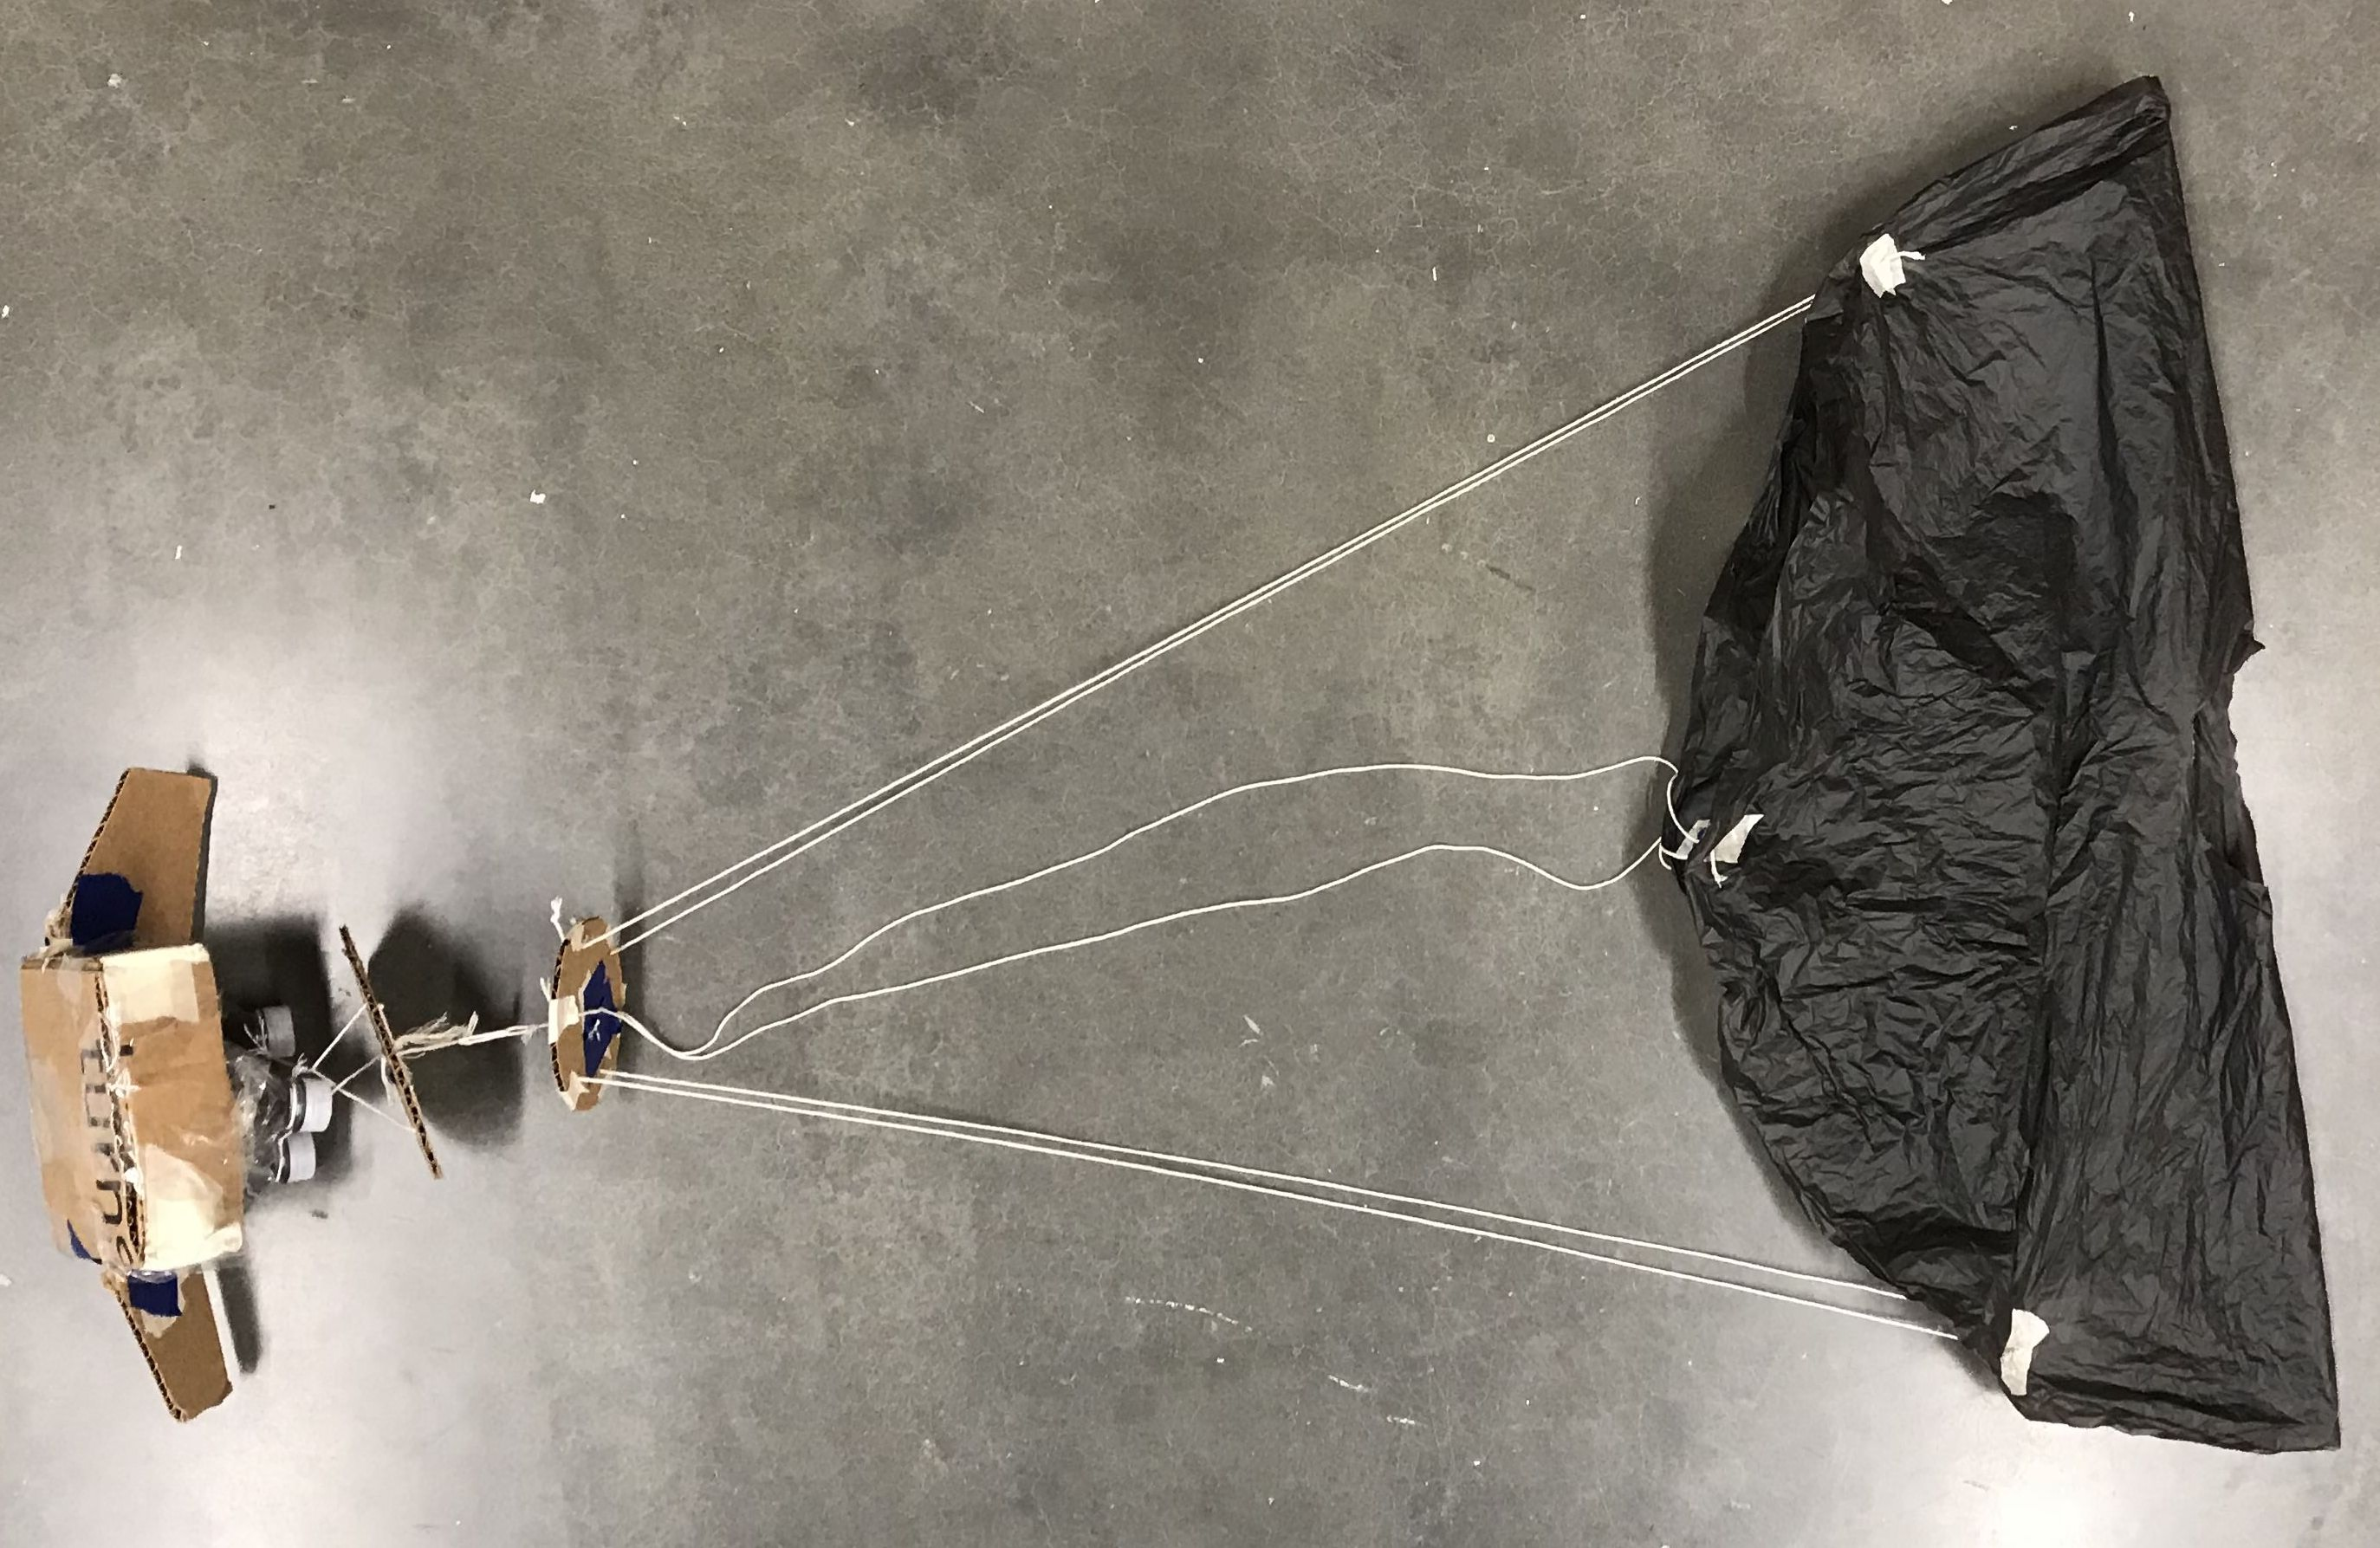
\includegraphics[width=90mm]{./figs/Parachute_Side.jpg}
\caption{A simple prototype of our parachute seen from the side.\label{overflow}}
\end{figure}

\begin{figure}[ht]
\centering
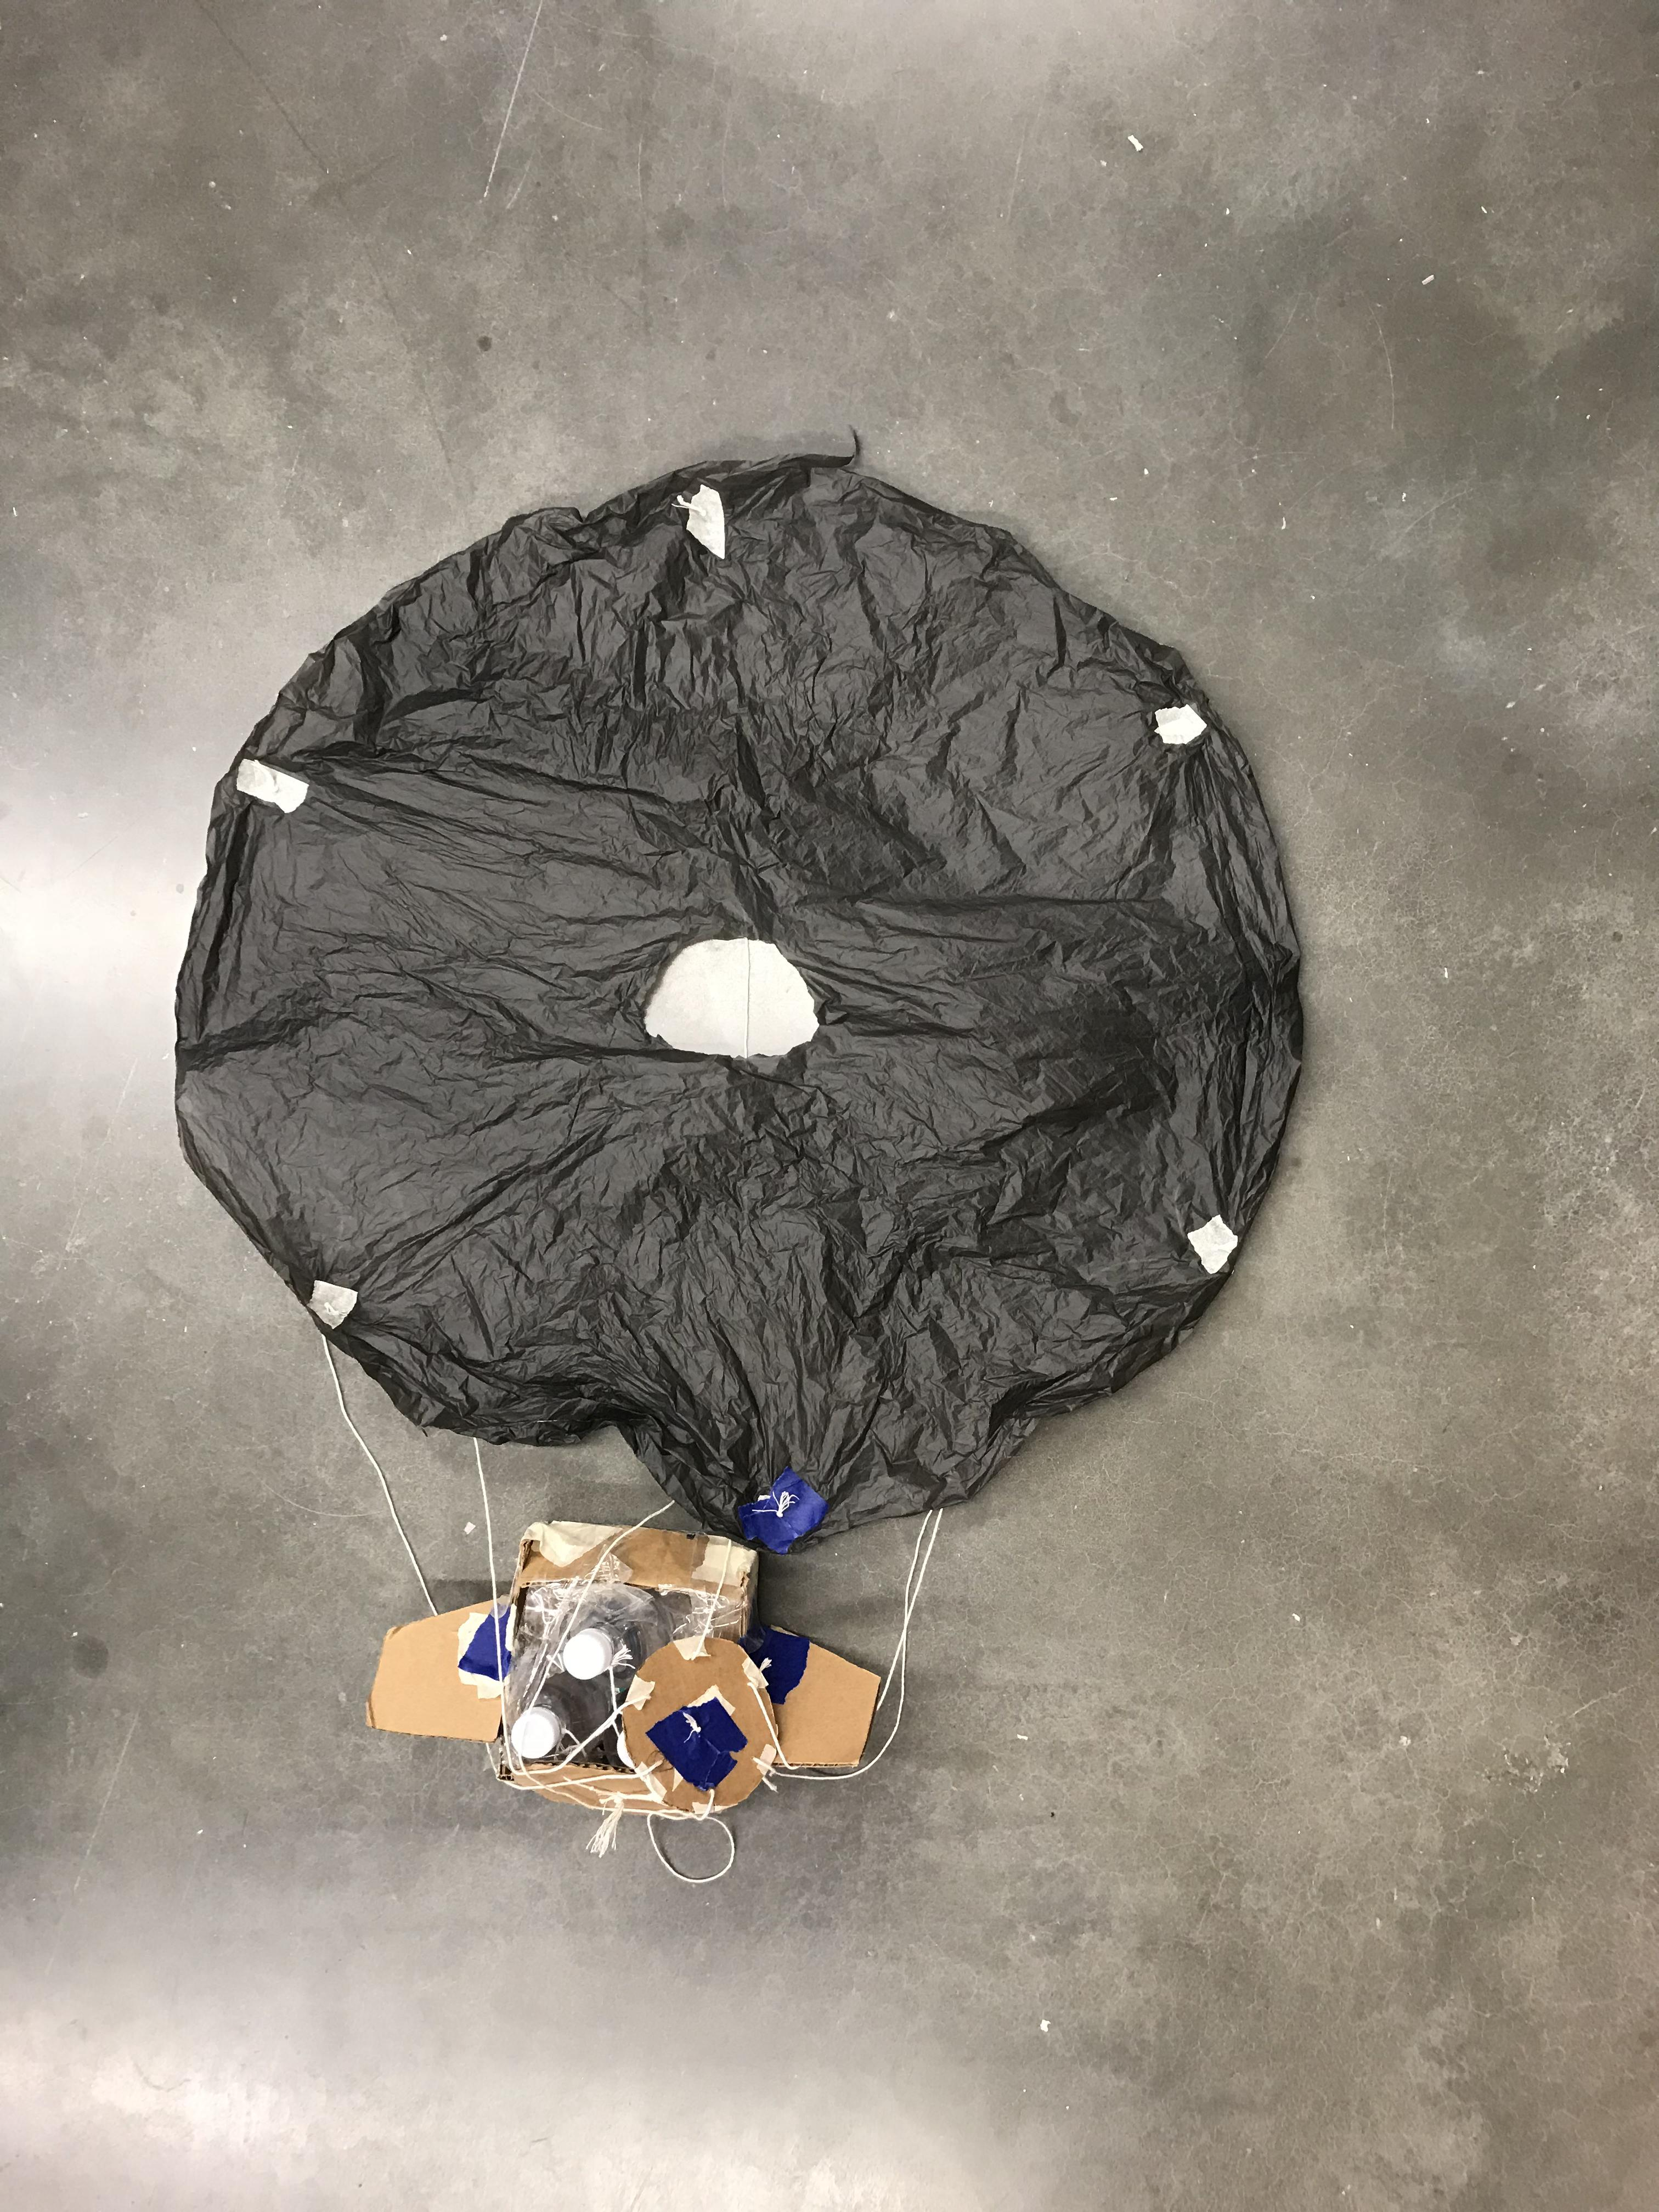
\includegraphics[width=90mm]{./figs/Parachute_Top.jpg}
\caption{A simple prototype of our parachute seen from the top. Note the hole in the middle of the parachute. As mentioned above, we found that this greatly improved the accuracy of the parachute. \label{overflow}}
\end{figure}

\begin{figure}[ht]
\centering
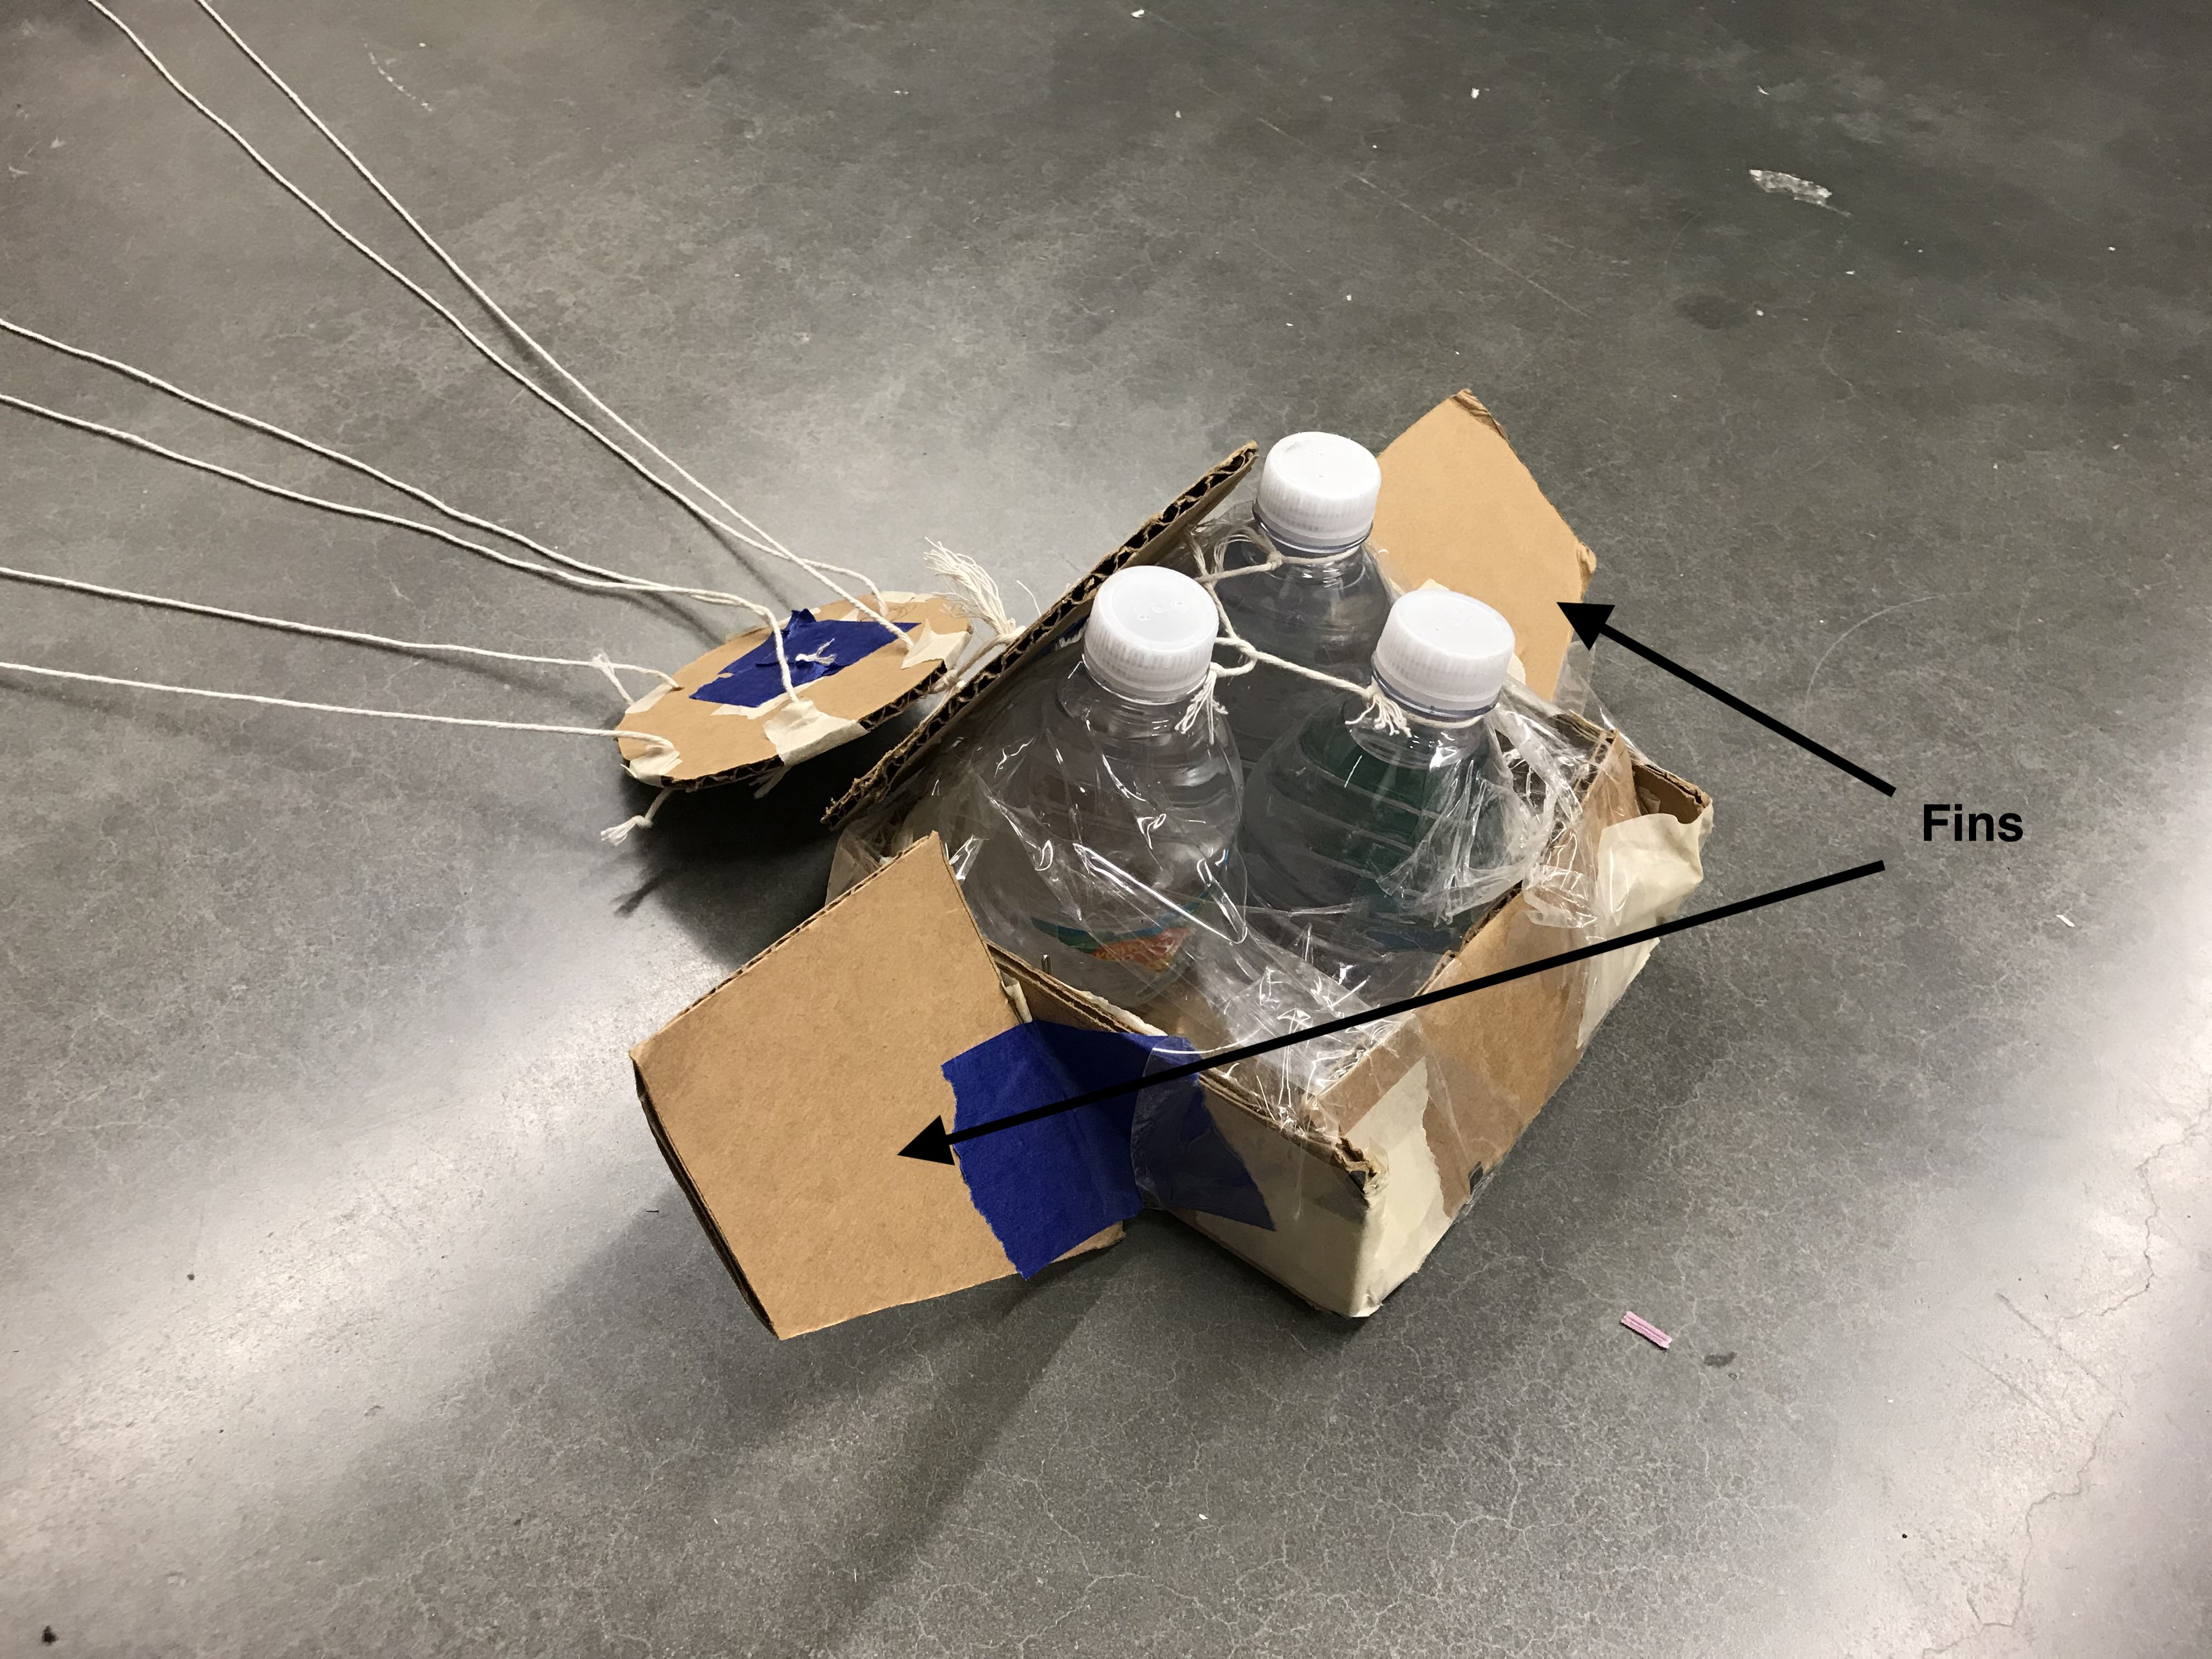
\includegraphics[width=90mm]{./figs/Parachute_Fins.jpg}
\caption{The payload we used to simulate the UGV. Note the fins. As mentioned above, preliminary results seem to indicate that these fins provided a small amount of control authority over the parachute's trajectory. This will help us improve accuracy \label{overflow}}
\end{figure}

\end{document}
